\section{Organizzazione del progetto}
\subsection{Ruoli e costi}
La seguente tabella riporterà i vari ruoli che i membri del gruppo \gruppo ~andranno a ricoprire durante lo svolgimento del progetto e i relativi costi orari:
\begin{center}
\centering
\begin{tabular}{| l | c |}
\hline
Ruolo & Costo orario \\
\hline
Responsabile & 30\euro \\
Amministratore & 20\euro \\
Analista & 25\euro \\
Progettista & 22\euro \\
Programmatore & 15\euro \\
Verificatore & 15\euro \\
\hline
\end{tabular}
\\
Tabella 1: costo orario per ruolo
\end{center}
I ruoli sono trattati in dettaglio in \VerbaleB.
Si ricorda inoltre che ogni membro del team dovrà ricoprire almeno una volta ogni ruolo disponibile durante lo svolgimento del progetto, facendo attenzione che non vi siano conflitti di interesse.
\subsection{Pianificazione}
Secondo il modello di ciclo di vita adottato, trattato in \ref{subsec:ciclodivita}, e le scadenze che il gruppo \gruppo ~intende rispettare riportate a \ref{subsec:Scadenze}, si è deciso di impostare lo sviluppo del progetto in quattro periodi fondamentali:
\begin{enumerate}
	\item Analisi (AN);
	\item Progettazione architetturale (PA);
	\item Progettazione di dettaglio e codifica (PDC);
	\item Validazione (VV).
\end{enumerate}
Ogni periodo è stato composto da vari processi i quali sono l'aggregazione di più attività, e lo svolgimento di queste verrà monitorato utilizzando dei diagrammi di Gantt forniti in automatico dallo strumento di ticketing come spiegato nelle \infoNDP. \\
Per ogni periodo verranno definiti gli obiettivi, quali per esempio il livello di maturità che i requisiti e la progettazione il team cercherà di raggiungere, evidenziando gli incrementi rilevanti che verranno apportati allo sviluppo del progetto al termine dei vari periodi.\\
Da notare che il processo di verifica è attivo durante l'intero svolgimento del progetto.\\
Per la pianificazione del progetto si è seguita la procedura rappresentata tramite il seguente diagramma di attività:
\newline
\newline
 \setlength{\unitlength}{1mm}\begin{picture}(0,29)
                \put(0,0){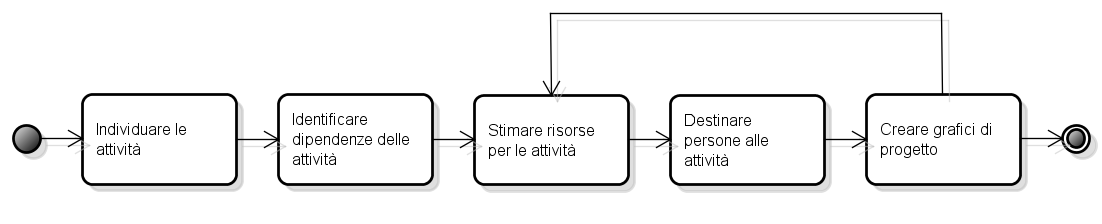
\includegraphics[scale=0.50]{../modello/img/pianificazione.png}}
        \end{picture}
\begin{center}
Diagramma di attività per la pianificazione di progetto.
\end{center}
l'attività di identificazione delle dipendenze necessita di particolare attenzione in quanto è necessario che vengano identificati i cammini critici, cioè quelle sequenze di attività con dipendenze funzionali critiche e dipendenze temporali strette. Ogni attività \textbf{critica} dovrà quindi essere classificata come tale nel caso in cui un suo ritardo crei un effetto di rallentamento o in generale dannoso per lo svolgimento di altre attività. Tali attività nella rappresentazione con il diagramma di Gantt verranno differenziate da quelle \textbf{non critiche} con il colore rosso.
\subsubsection{Analisi}
Questo periodo si è esteso per 28 giorni, dal \textit{2014-02-05} al \textit{2014-03-05} ed i ruoli che sono stati maggiormente coinvolti sono: \textit{Responsabile}, \textit{Amministratore} e \textit{Analista}.
In questo periodo si è cercato di lavorare a stretto contatto per instaurare un rapporto di fiducia tra i membri del \textit{team} creando un ambiente di fiducia comunicando apertamente.
\\
Il gruppo \gruppo ha lavorato per poter presentare i seguenti documenti alla consegna del \textit{2014-03-05}:
\begin{itemize}
	\item \textbf{Norme di progetto:} documento che dovrebbe essere redatto a "tempo zero", viene steso dall'\textit{amministratore} e fissa regole, procedure e strumenti funzionali al raggiungimento degli obiettivi strategici. Tale documento è stato steso prima di ogni altro in quanto vincola le modalità di stesura, e non solo, di tutti gli altri documenti che dovranno essere prodotti. Per questo motivo le attività ad esso correlate saranno critiche.
	\\ Il rispetto di tali norme verrà attestato dai verificatori;
	\item \textbf{Studio di Fattibilità:} l'\textit{analista} designato valuta i vari capitolati d' appalto forniti e ne analizza vari fattori: complessità~, vantaggi, svantaggi e interesse nel suo svolgimento. Le attività del processo di stesura di questo documento sono critiche in quanto senza di esso non si può procedere con l'analisi dei requisiti;
	\item \textbf{Analisi dei requisiti:} l'attività di stesura di questo documento ha termine solo se il documento supera con successo la revisione di progettazione. Durante il periodo di analisi si cercherà di identificare al meglio i requisiti del sistema;
	\item \textbf{Piano di progetto:} Il \textit{Responsabile} per mezzo di questo documento fissa le risorse disponibili, la suddivisione delle attività ed il calendario ad esse connesso; 
	\item \textbf{Piano di qualifica:} Questo documento fissa le strategie di verifica del gruppo e viene redatto dall'\textit{Analista} con la stretta collaborazione del \textit{Responsabile} e dell'\textit{Amministratore} per la sua buona stesura;
	\item \textbf{Glossario:} Scritto e mantenuto costantemente aggiornato dai membri del gruppo contenente termini ambigui o poco chiari, necessari per la corretta interpretazione dei documenti;
	\item \textbf{Lettera di presentazione:} Documento necessario per permettere al gruppo di partecipare alla gara d' appalto, il destinatario è il committente.
\end{itemize}
Per quanto concerne l'attività di verifica, al completamento di un documento oppure quando richiesto dal redattore dello stesso, ogni documento verrà verificato da un \textit{verificatore} per accertarsi della sua correttezza.\\
Al termine di questo periodo il team \gruppo cercherà di avere i requisiti tra \textit{bounded} e \textit{acceptable}.\\
 \setlength{\unitlength}{1mm}\begin{picture}(0,70)
                \put(0,0){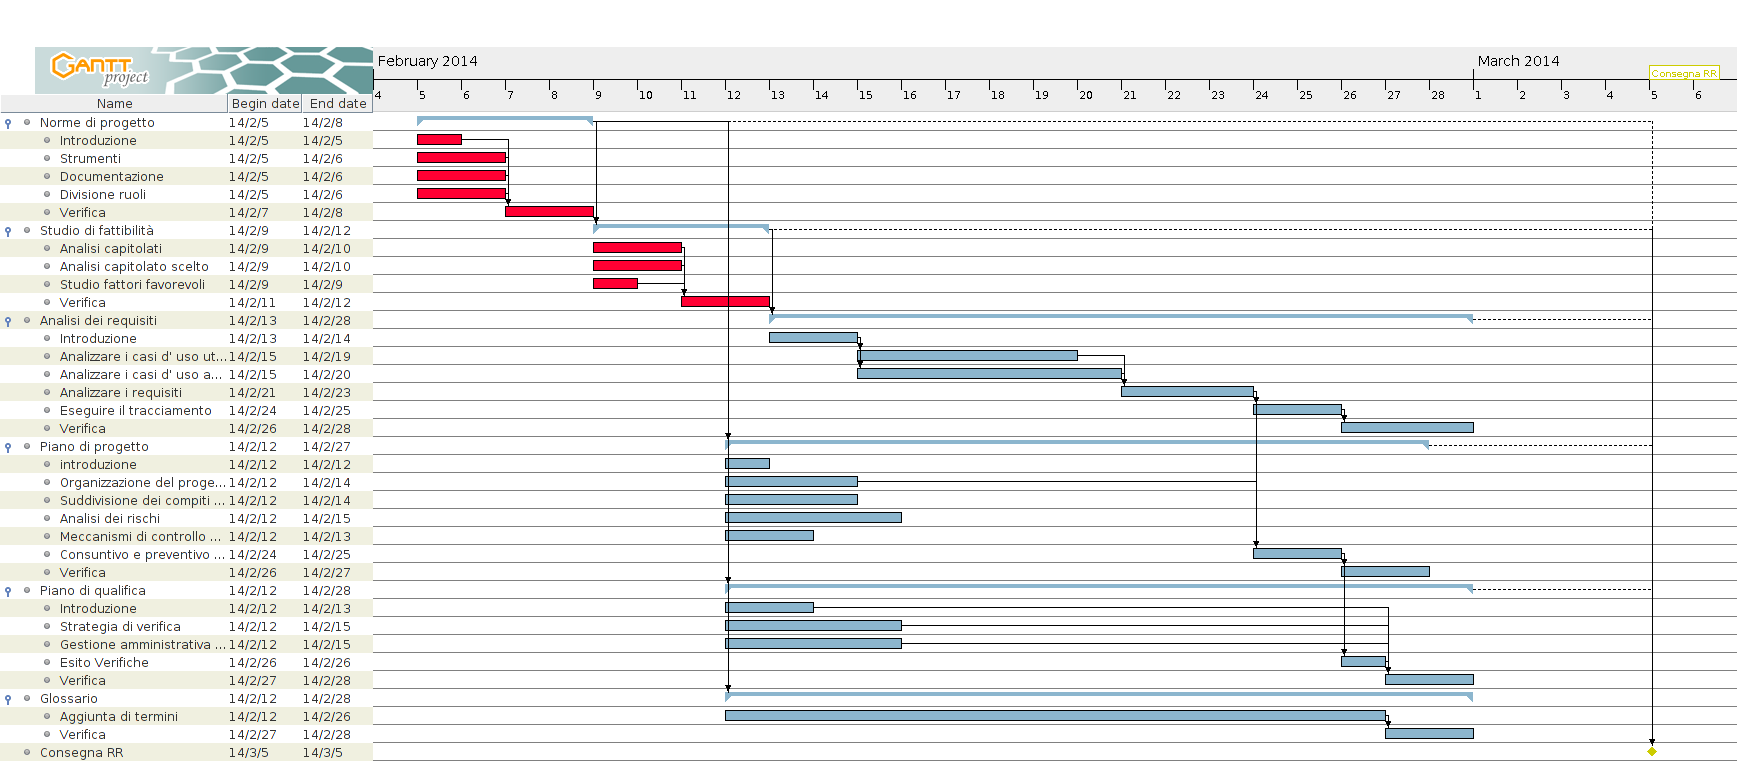
\includegraphics[scale=0.25]{../modello/img/RR.png}}
        \end{picture}
\begin{center}
Immagine 1: Diagramma di Gantt, periodo di Analisi
\end{center}
\subsubsection{Progettazione Architetturale}
Questo periodo si è esteso per 18 giorni, dal \textit{2014/03/11} al \textit{2014/03/29} ed i ruoli che saranno maggiormente attivi saranno: \textit{Responsabile}, \textit{Amministratore}, \textit{Progettista}, \textit{Verificatore} e \textit{Analista}. Nel primo intervallo di questo periodo il team andrà a correggere gli errori segnalati all'uscita dalla \textbf{RR}\ped{G} ponendo particolare attenzione all'analisi dei requisiti in quanto sarà con molta probabilità da correggere e necessiterà di incremento; solo successivamente si potrà andare a incrementare i documenti già esistenti e a stendere la \textbf{Specifica  Tecnica} che rappresenta il principale incremento apportato allo sviluppo del progetto durante questo periodo. Tale documento, redatto dal \textit{Progettista}, conterrà una modellazione del sistema \textit{Software} con una prima caratterizzazione architetturale dei componenti.\\
Per quanto concerne l'attività di verifica, al completamento di un documento oppure quando richiesto dal redattore dello stesso, ogni documento verrà verificato da un \textit{verificatore} per accertarsi della sua correttezza.\\
Al termine di questo periodo il team si impegna ad avere i requisiti tra uno stato di \textit{acceptable} e \textit{addressed} mentre di avere una progettazione ad un livello di \textit{architecture selected}, questi sono dati dal fatto che si svolgerà un' analisi di alto livello.\\
 \setlength{\unitlength}{1mm}\begin{picture}(0,72)
                \put(0,0){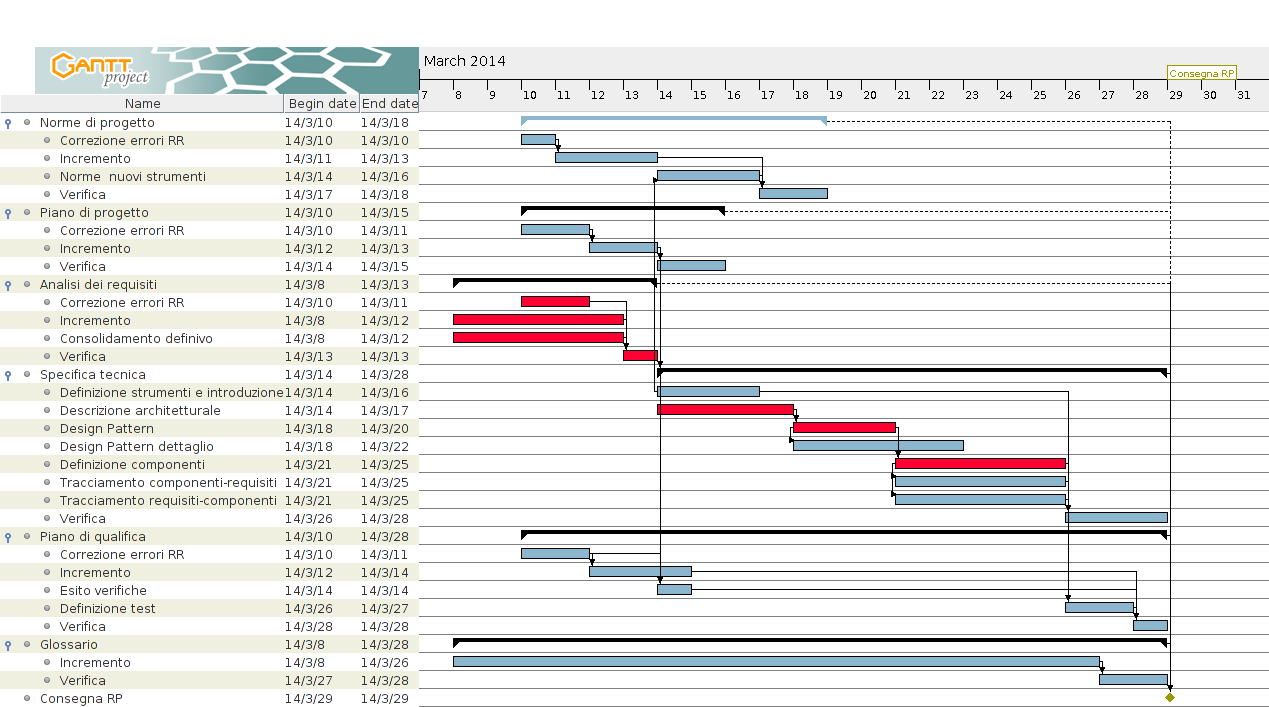
\includegraphics[scale=0.30]{../modello/img/RP.png}}
        \end{picture}
\begin{center}
Immagine 2: Diagramma di Gantt, periodo di Progettazione Architetturale
\end{center}
\subsubsection{Progettazione di Dettaglio e Codifica}
Periodo che si estende dal \textit{2014-04-14} al \textit{2014-06-28}. Durante questo lasso di tempo i ruoli maggiormente coinvolti saranno: \textit{Progettista}, \textit{Programmatore} e \textit{Verificatore}. I documenti prodotti in questo periodo saranno:
\begin{itemize}
	\item \textbf{Definizione di Prodotto}: rappresenta l'incremento più importante apportato da questo periodo, il documento definisce nel dettaglio la struttura del sistema per fornire una struttura dettagliata che verrà poi utilizzata dai \textit{programmatori} per la codifica. I suoi contenuti si baseranno su quanto presente nella \textit{Specifica Tecnica};
	\item \textbf{Manuali utente} Questi documenti saranno utilizzati dagli utenti del sistema per ottenere informazioni sull'utilizzo del \progetto , venendo stesi per la prima volta in questo periodo ne definiscono una parte dell'incremento apportato allo sviluppo del progetto.
\end{itemize}
Dovranno essere inoltre essere eseguite le seguenti attività~:
\begin{itemize}
\item \textbf{Codifica:} i programmatori basandosi su quanto riportato nella \textit{Definizione di Prodotto} forniranno una versione del sistema funzionante, la quale sarà certamente un incremento significativo che il team intende apportare al progetto in quanto utile anche per ricevere pareri e impressioni dal proponente inoltre, dopo aver prodotto una prima versione con le funzionalità base implementando i requisiti base, si andranno a eseguire i vari incrementi aggiungendo nuove funzionalità;
\item \textbf{Test} Si eseguiranno i test pianificati e si analizzeranno i risultati ottenuti.
\end{itemize}
Per quanto concerne l'attività di verifica, quando un documento sarà pronto, o quando chi lo redige lo riterrà necessario, i documenti verranno verificati per verificarne la correttezza inoltre anche il codice prodotto dovrà essere verificato.\\
Al termine di questo periodo oltre ai documenti prodotti e alla codifica effettuata, si cercherà di avere i requisiti ad uno stato almeno \textit{addressed} e un livello di progettazione e codifica \textit{usable}.\\
 \setlength{\unitlength}{1mm}\begin{picture}(0,46)
                \put(10,0){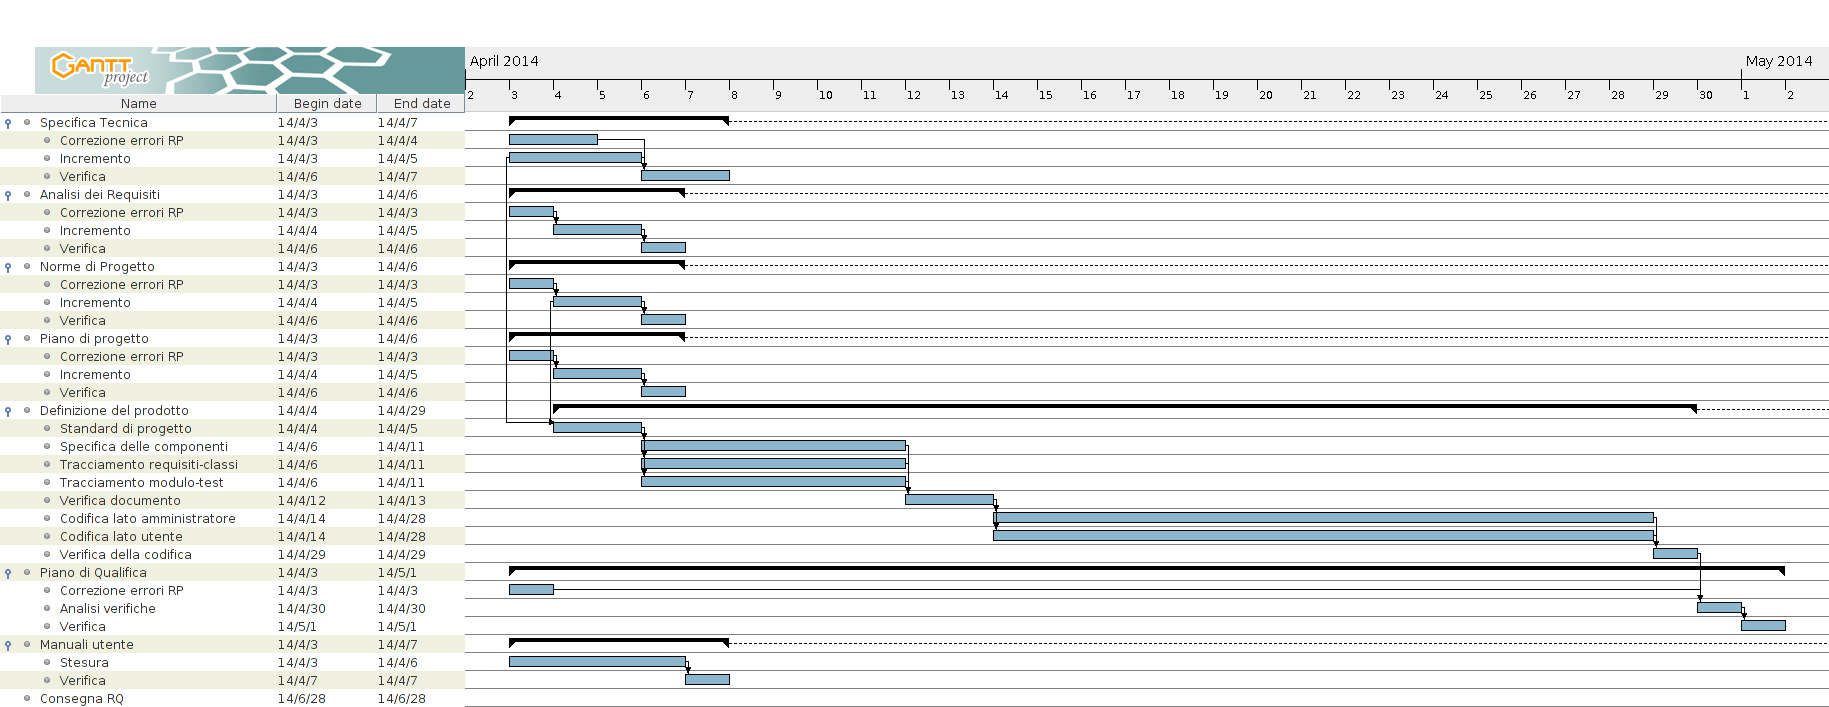
\includegraphics[scale=0.19]{../modello/img/RQ.png}}
        \end{picture}
        \begin{center}
Immagine 3: Diagramma di Gantt, periodo di Progettazione di Dettaglio e Codifica
\end{center}
\subsubsection{Validazione}
Dal \textit{2014-07-03}  \textit{2014-07-18} il gruppo lavorerà per terminare il processo di sviluppo del \textit{software}. In questo periodo si dovranno eseguire le seguenti attività:
\begin{itemize}
	\item \textbf{Incremento e verifica finali: } I documenti riceveranno le ultime modifiche e poi dovranno essere verificati e validati;
	\item \textbf{Codifica:} In base alle ultime modifiche effettuate alla \textit{Definizione di Prodotto}, in seguito ai \textit{feedback} del proponente, si dovrà produrre la versione corrispondente del sistema e verificarne la correttezza;
	\item \textbf{Test e collaudo:} Si effettueranno gli ultimi test sul sistema per assicurarsi il suo corretto funzionamento e il collaudo generale, testandone le funzionalità cercando di raggiungere quanti più obiettivi qualitativi possibili.
\end{itemize}
Al termine della RA il gruppo si impegna ad aver raggiunto un livello di maturità dei requisiti \textit{fulfilled} e di progettazione e codifica di \textit{ready}.\\
 \setlength{\unitlength}{1mm}\begin{picture}(0,87)
                \put(0,0){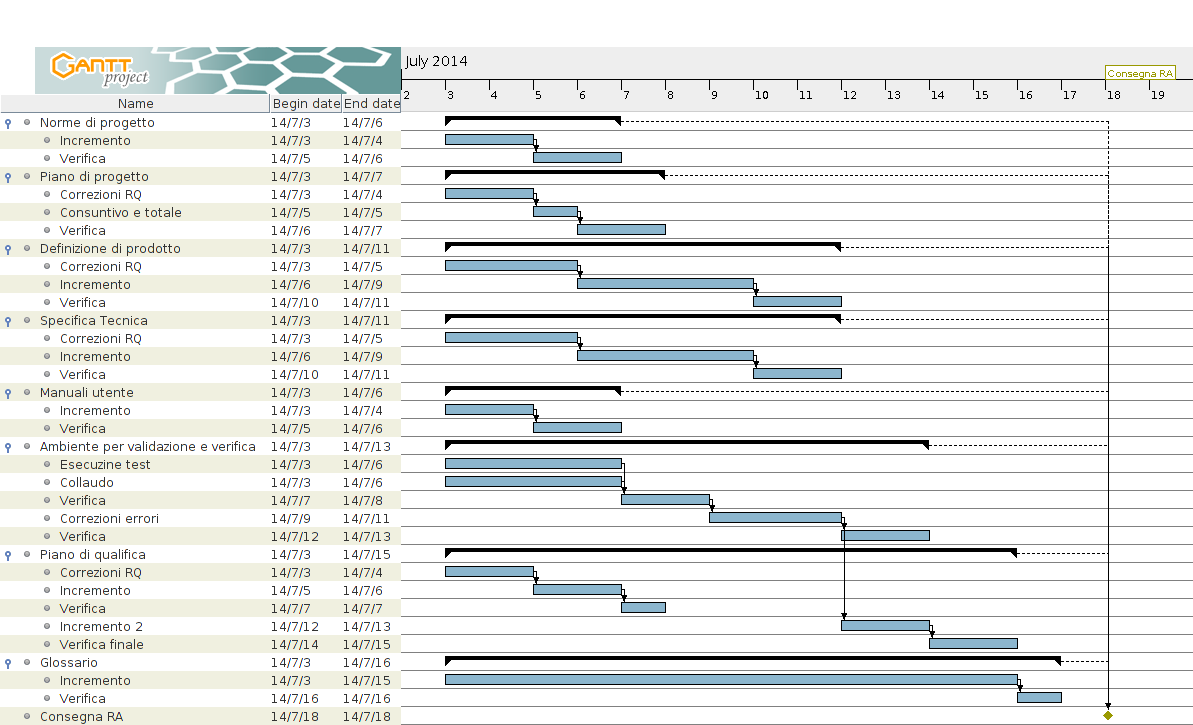
\includegraphics[scale=0.35]{../modello/img/RA.png}}
        \end{picture}
        \begin{center}
Immagine 4: Diagramma di Gantt, periodo di Verifica e Validazione
\end{center}